                               %----------------------------------%
                               % Manhattan College Math Dept      %
                               % Student Homework Template v1     %
                               %    R. Goldstone, 1/1/2011        %
 	               % Edited by T. McGrail, 2/11/2011  %
 	               % Edited by R. McGovern, 8/16/2011 %
 	               % Edited by J. Kirtland, 1/20/2015 %
                               %----------------------------------%
% PREAMBLE ============================================================================

\documentclass[12pt]{article}
\usepackage[utf8]{inputenc}    % set input encoding so bullets are printed
\usepackage{amssymb,amsmath,amsthm}
\usepackage{listings}
\usepackage[usenames,dvipsnames]{color}
\usepackage{matlab-prettifier}
\usepackage{graphicx}

 
% FILL-IN, THEN GO TO DOCUMENT MAIN BODY **********************************************
% TEXWORKS: USE CTRL-TAB TO JUMP FROM INPUT FIELD TO INPUT FIELD
\newcommand{\myname}{Amy Pitts} % Enter name
\newcommand{\duedate}{February 30, 2019} % Enter date, e.g., April 1
\newcommand{\courseno}{440L}      % Enter course number (just the number)
\newcommand{\coursename}{Machine Learning}    % Enter course name
\newcommand{\instructorname}{Instructor: Dr. Pablo Rivas} % Enter instructor name
\newcommand{\assignumber}{2}   % Enter assignment number#.
\newcommand{\exerciselist}{Chapter 2,3}      % Enter problem references.  Give a complete list, in order, of all of the problems that you will do on this assignment.  Use the format 2.20 to designate problem  # 20 from chapter 2 of the text.
\newcommand{\spacingfactor}{2}
% END FILL-IN *************************************************************************

% DOCUMENT STRUCTURES -----------------------------------------------------------------

% PAGES
\usepackage[paper=letterpaper, margin=1in, headsep=20pt]{geometry}
  
\newcommand{\firstpageinfo}  
    {\textsf{\large\myname}    \hfill     Math \courseno{:}\,\coursename \\
  Assignment Number \assignumber \hfill  Due:  \duedate \\
  \instructorname}
% END PAGES

% HEADERS AND FOOTERS
\usepackage{fancyhdr}
\pagestyle{fancy}              % Headers and footers for page 2 and beyond
  \lhead{\textit{\myname}}
  \chead{\textit{Math \courseno}}
  \rhead{\textit{\textit{Assignment Number \assignumber}}}
  \cfoot{\textit{\thepage}}
  \renewcommand{\headrulewidth}{0.4pt}
% END HEADERS AND FOOTERS

% TEXT SPACING
\usepackage{setspace}   %Allows for Doublespacing
\usepackage{ifthen}   %Used to create a response environment
% END TEXT SPACING

% PROBLEM AND RESPONSE ENVIRONMENTS
 \newcommand\myqed{}                 % creates command for tombstone at end of proof
\newcommand{\printmyqed}[1][]       % decides whether to print tombstone or not
  {%
  \ifthenelse{\equal{#1}{Proof}}
  {\renewcommand{\myqed}{\qed}}
  {\renewcommand{\myqed}{}}
  }

\newenvironment{exercise}[1][]{%
  \bigskip                          % Space before problem statement
  \noindent \textsf{Exercise #1.}\slshape }{}
   
\newenvironment{response}[1][\textit{Solution}]{%
  \printmyqed[#1]
  \begin{spacing}{\spacingfactor}
  \medskip                          % Space before solution
  \noindent \textit{#1.}}{\myqed\end{spacing}\medskip\hrule}
% END PROBLEM AND RESPONSE ENVIRONMENTS

% =====================================================================================

\begin{document}
\thispagestyle{empty}

% TOP MATTER --------------------------------------------------------------------------
\noindent\firstpageinfo
\begin{center} \underline{\textsf{Exercise List}}\\[5pt] \exerciselist \end{center}
\medskip\hrule
% END TOP MATTER ----------------------------------------------------------------------


%----------------------------------------------------------------------------------------
\begin{exercise}[2.1] % Put problem reference inside the brackets
In Equestion (2.1), set $\delta=0.03$ and let 
\begin{equation*}
  \epsilon(M,N,\delta) = \sqrt{\frac{1}{2N}\ln\frac{2M}{\delta}}.
\end{equation*}
\begin{enumerate}
  \item[a)] For $M=1$, how many examples do we need to make $\epsilon \leq 0.05$?
  \item[b)] For $M=100$, how many examples do we need to make $\epsilon \leq 0.05$?
  \item[c)] For $M=10,000$, how many examples do we need to make $\epsilon \leq 0.05$? 
\end{enumerate}
\end{exercise}
  
  
\begin{response}[Solution]
\textbf{a)} We want to obtain $ \sqrt{\frac{1}{2N}\ln\frac{2M}{\delta}} \leq 0.05$. 
Using the information provided we have $ \sqrt{\frac{1}{2N}\ln\frac{2}{0.03}} \leq 0.05$. 
Solving for $N$ we get 
\begin{align*}
  \sqrt{\frac{1}{2N}\ln\frac{2}{0.03}} &\leq 0.05 \\
  \frac{1}{2N}\ln\frac{2}{0.03} &\leq 0.0025 \\
  \frac{1}{2N}(\ln2 - \ln0.03) &\leq 0.0025 \\
  \frac{1}{2N} &\leq \frac{0.0025}{(\ln2 - \ln0.03)} \\
  2N &\geq \frac{\ln2 - \ln0.03}{0.0025} \\
  N &\geq \frac{\ln2 - \ln0.03}{0.005} \\
  N &\geq 839.941.
\end{align*}
Thus, $N=840$ when $M=1$. 

\textbf{b)} We want to obtain $ \sqrt{\frac{1}{2N}\ln\frac{2M}{\delta}} \leq 0.05$. 
Using the information provided we have $ \sqrt{\frac{1}{2N}\ln\frac{200}{0.03}} \leq 0.05$. 
Solving for $N$ with the same steps above we obtain 
\begin{align*}
  \sqrt{\frac{1}{2N}\ln\frac{200}{0.03}} &\leq 0.05 \\
  N &\geq \frac{\ln200 - \ln0.03}{0.005} \\
  N &\geq 1760.98.
\end{align*}
Thus, $N=1761$ when $M=100$. 

\textbf{b)} We want to obtain $ \sqrt{\frac{1}{2N}\ln\frac{2M}{\delta}} \leq 0.05$. 
Using the information provided we have $ \sqrt{\frac{1}{20N}\ln\frac{20000}{0.03}} \leq 0.05$. 
Solving for $N$ with the same steps above we obtain 
\begin{align*}
  \sqrt{\frac{1}{2N}\ln\frac{20000}{0.03}} &\leq 0.05 \\
  N &\geq \frac{\ln20000 - \ln0.03}{0.005} \\
  N &\geq 2682.01.
\end{align*}
Thus, $N=2683$ when $M=10,000$. 
\end{response}
%------------------------------------------------------


\begin{exercise}[2.11] % Put problem reference inside the brackets
Suppose $m_H(N)=N+1$, so $d_{VC}=1$. You have 100 training examples. 
Use the generalization bound to give a bouond for $E_{out}$ with 
confidence $90\%$ . Repeat for $N=10,000$. \\
  Hint: you should use equation (2.12) and remember that a confidence
of 90\% means a $\delta=0.1$. 
\end{exercise}
   
\begin{response}[Solution] 
$E_{out}(g)\leq E_{in}(g)+\sqrt{\frac{8}{N}\ln\frac{4m_H(2N)}{\delta}}$
plugging in information we have 
\begin{align*}
  E_{out}(g)&\leq E_{in}(g)+\sqrt{\frac{8}{100}\ln\frac{4m_H(200)}{0.1}}\\
  &=E_{in}(g)+\sqrt{\frac{8}{100}\ln\frac{4(200+1)}{0.1}} \\
  &=E_{in}(g)+\sqrt{\frac{8}{100}\ln\frac{804}{0.1}} \\
  &=E_{in}(g)+0.8481596 \\
\end{align*}
When $N=10000$ we have 
\begin{align*}
  E_{out}(g)&\leq E_{in}(g)+\sqrt{\frac{8}{10000}\ln\frac{4m_H(20000)}{0.1}}\\
  &=E_{in}(g)+\sqrt{\frac{8}{10000}\ln\frac{4(20000+1)}{0.1}} \\
  &=E_{in}(g)+\sqrt{\frac{8}{10000}\ln\frac{80004}{0.1}} \\
  &=E_{in}(g)+0.1042782\\
\end{align*}

\end{response}


%------------------------------------------------------

\begin{exercise}[2.12] % Put problem reference inside the brackets
For an $H$ with $d_{VC}=10$, what sample size do you need 
(as prescribed by the generalization bound) to have a 95\% confidence
that your generalization error is at most 0.05? \\
  Hint: Use Equation (2.13) 
\end{exercise}
   
\begin{response}[Solution] 
  Using the equation $N \geq \frac{8}{\epsilon^2}\ln \left(\frac{4(2N)^{d_{vc}}+1}{\delta}\right)$
  and plugging in we have 
  \begin{align*}
    N &\geq \frac{8}{\epsilon^2}\ln \left(\frac{4(2N)^{d_{vc}}+1}{\delta}\right) \\
    &= \frac{8}{0.05^2}\ln \left(\frac{4(2N)^{10}+1}{0.05}\right) \\
    &= 3200\ln \left(81920N^{10}+20\right)
  \end{align*}
  We want to find the $N$ which makes the equation true. 
  \lstinputlisting[language=Python,frame=single]{q2_12.py}
  Using the code above the optimal number for $N$ is 
  452957 rounding up when comparing 8 decimal places. 
\end{response}

%------------------------------------------------------


\begin{exercise}[3.1] % Put problem reference inside the brackets
Consider the double semi-circle "toy" learning task below. \\
There are two semi-circles of width \textit{thk} with inner radius
\textit{rad}, separated by \textit{sep} as shown (red is -1 and blue is +1).
The center of the top semi-circle is aligned with the middle of the 
edge of the bottom semi-circle. This task is linearly separable when 
\textit{sep} $\geq0$, and not so for \textit{sep} $<0$. Set \textit{rad}=10
\textit{thk}=5 and \textit{sep}=5. Then, generate 2,000 examples 
uniformly, which means you will have approximately 1,000 examples for each class 
\begin{enumerate}
  \item[a)] Run the PLA starting from $w=0$ until it converges. Plot the
  data and the final hypothesis.  
  \item[b)] Repeat part (a) using the linear regression (for classification) 
  to obtain $w$. Explain your observations.  
\end{enumerate}
Use the dataset generator downloadable on Ilearn. 
\end{exercise}
   
\begin{response}[Solution] 
\textbf{a)} The PLA took 5 iteration before it found the ideal line.\\
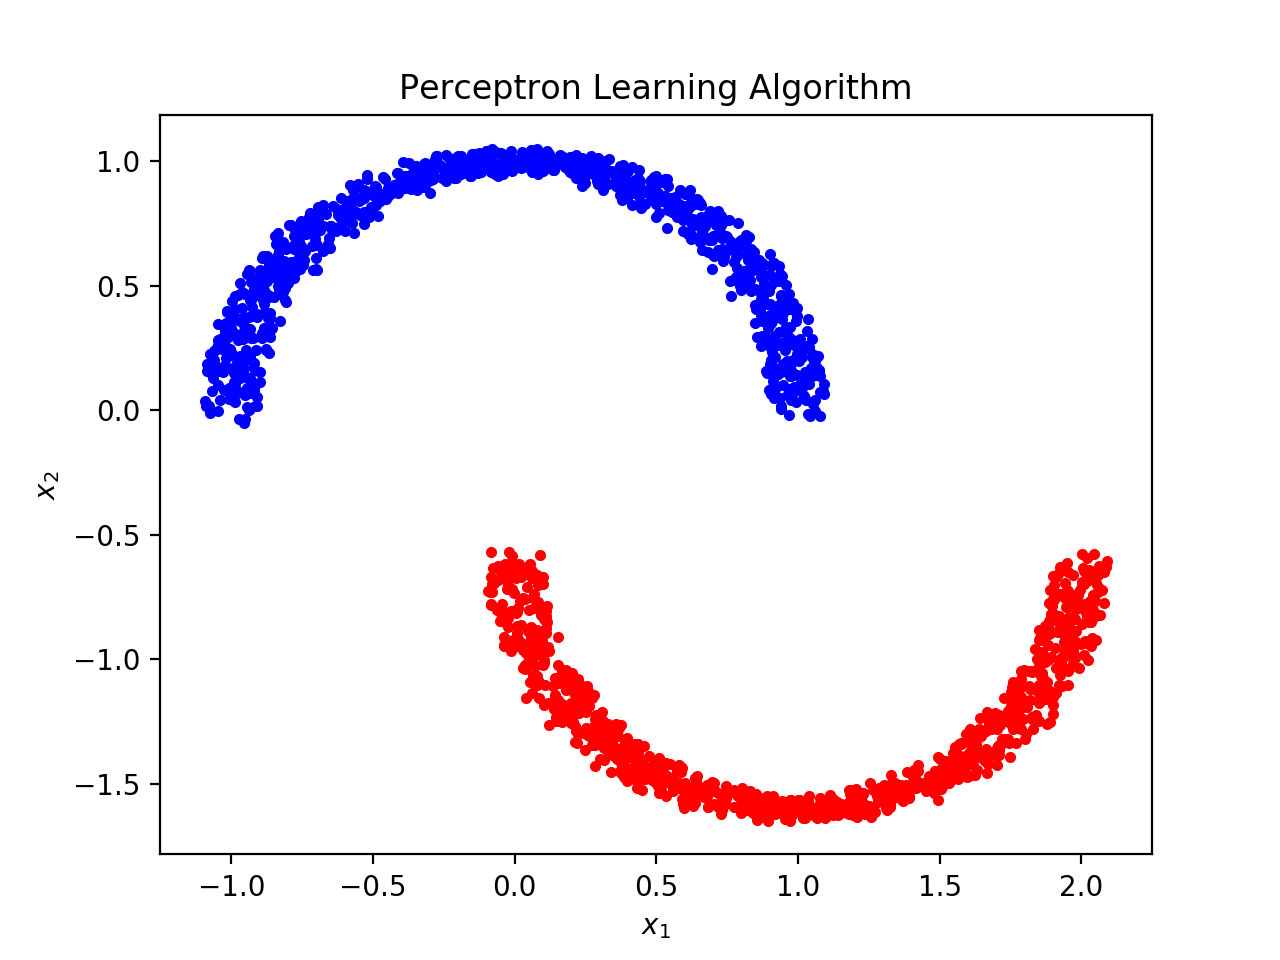
\includegraphics[width=85mm]{3a_3.png} 
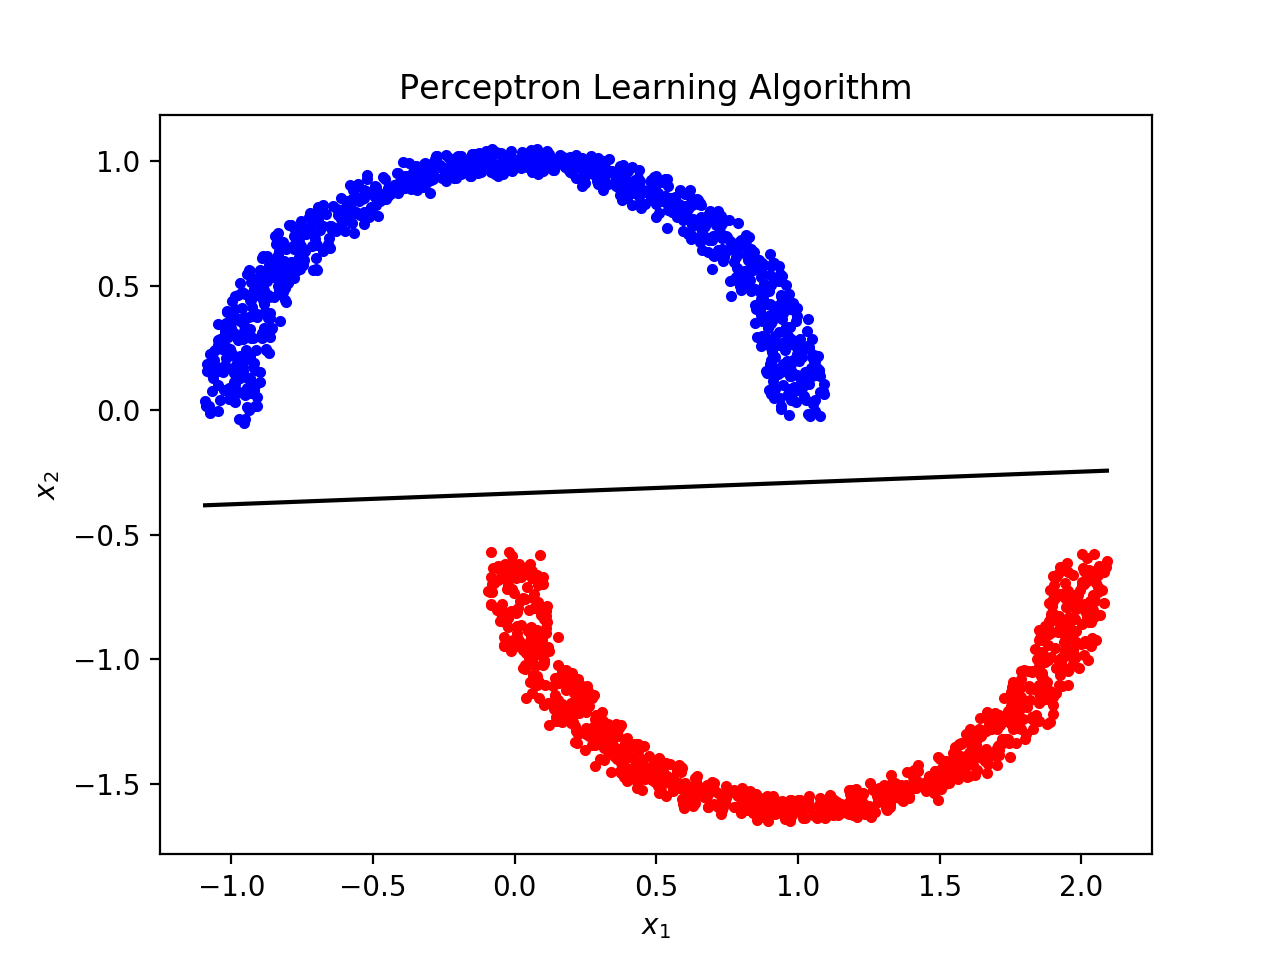
\includegraphics[width=85mm]{3a_4.png} 
\\
\textbf{b)} When starting the PLA off with linear regression 
it took zero iterations to find a line that works. Curious
to see if what would happen I ran this function several more 
times and every time it took it 0 iterations to find the correct 
line. Therefore, starting with linear regression can decrease 
run time because it helps the pla converge faster.  The code 
used to replace the vector of zeros is listed below. \\
\lstset{language=Matlab,breaklines=true,basicstyle=\small\ttfamily}
  \begin{lstlisting}[language=Python,frame=single]
    #linear regression
    Xs = np.linalg.pinv(X.T.dot(X)).dot(X.T) 
    wlr = Xs.dot(y)
    # initialize the weigths to linear regression 
    w = wlr
  \end{lstlisting}
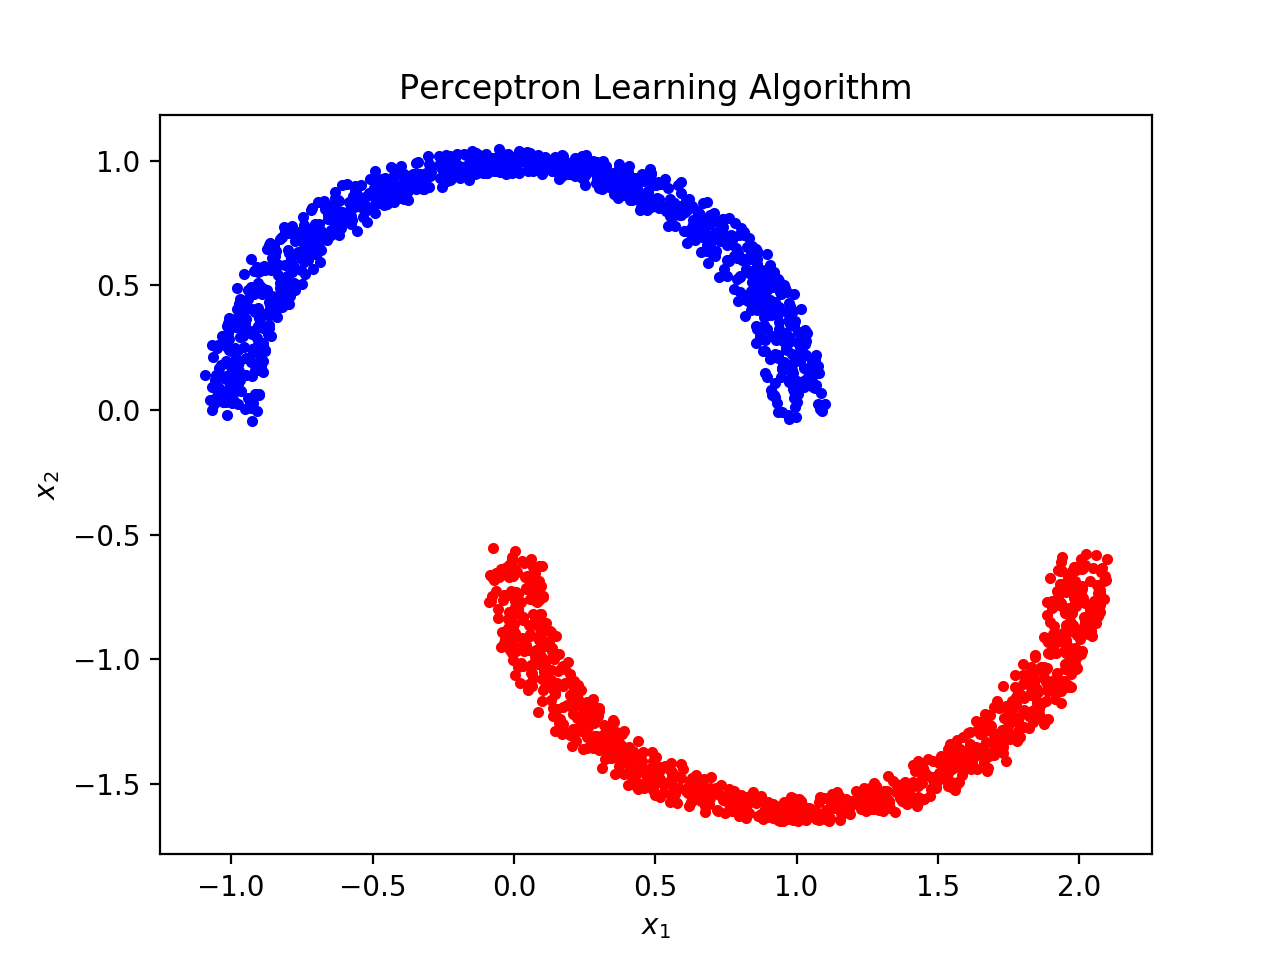
\includegraphics[width=85mm]{3b_2.png} 
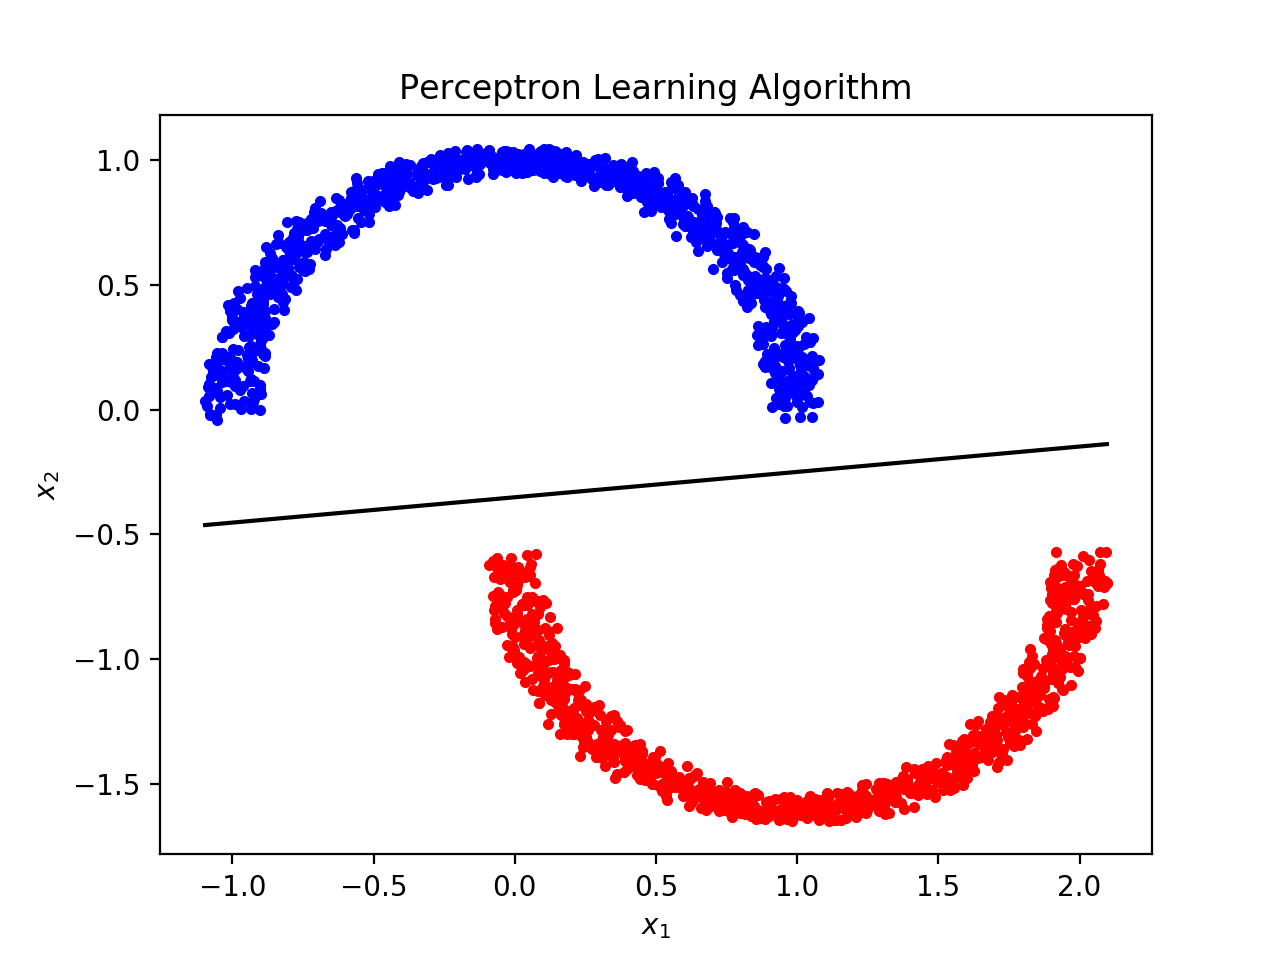
\includegraphics[width=85mm]{3b_1.png} 
\end{response}


%------------------------------------------------------


\begin{exercise}[3.2] % Put problem reference inside the brackets
\textbf{Extra Credit } For the double-semi-circle task in Problem 3.1,
vary \textit{sep} in the range $\{0.2,0.4,\dots,5\}$. Generate 2,000 examples 
and run the PLA starting with $w=0$. Record the number of iterations PLA
takes to converge. \\
Plot \textit{sep} versus the number of iterations taken for PLA to converge. 
Explain your observations \\
Hint: Problem 1.3 
\end{exercise}
   
\begin{response}[Solution]  The bigger the sep number the less iterations it takes 
  to find the optimal line to split the data. There seems
  to be a general trend from left to right of the number 
  of iterations goes down as the sep length increase. 

  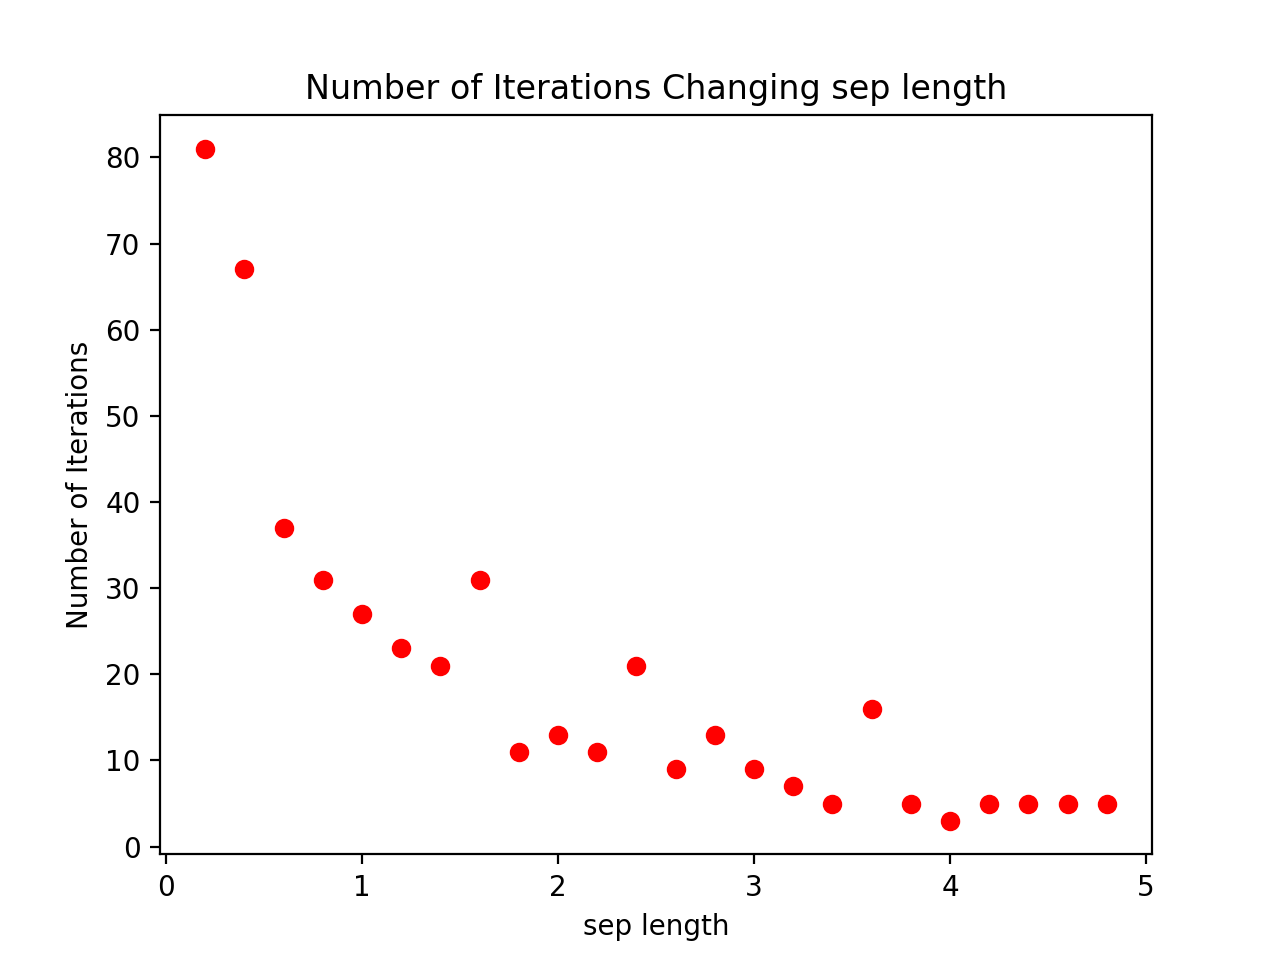
\includegraphics[width=150mm]{3_2_plot.png} 

\end{response}


\end{document}
%======================================================================================
% END DOCUMENT MAIN BODY ==============================================================
% COPY AND PASTE THIS DOUBLE-SPACE PROBLEM-RESPONSE PAIR AS NEEDED
%======================================================================================



